%%%%%%%%%%%%%%%%%%%%%%%%%%%%%%%%%%%%%%%%%
% a0poster Landscape Poster
% LaTeX Template
% Version 1.0 (22/06/13)
%
% The a0poster class was created by:
% Gerlinde Kettl and Matthias Weiser (tex@kettl.de)
% 
% This template has been downloaded from:
% http://www.LaTeXTemplates.com
%
% License:
% CC BY-NC-SA 3.0 (http://creativecommons.org/licenses/by-nc-sa/3.0/)
%
%%%%%%%%%%%%%%%%%%%%%%%%%%%%%%%%%%%%%%%%%

%----------------------------------------------------------------------------------------
%	PACKAGES AND OTHER DOCUMENT CONFIGURATIONS
%----------------------------------------------------------------------------------------

\documentclass[a0,landscape]{a0poster}
\usepackage{cite}



\usepackage{multicol} % This is so we can have multiple columns of text side-by-side
\columnsep=100pt % This is the amount of white space between the columns in the poster
\columnseprule=3pt % This is the thickness of the black line between the columns in the poster

\usepackage[svgnames]{xcolor} % Specify colors by their 'svgnames', for a full list of all colors available see here: http://www.latextemplates.com/svgnames-colors

\usepackage{times} % Use the times font
%\usepackage{palatino} % Uncomment to use the Palatino font

\usepackage{graphicx} % Required for including images
\graphicspath{{figures/}} % Location of the graphics files
\usepackage{booktabs} % Top and bottom rules for table
\usepackage[font=small,labelfont=bf]{caption} % Required for specifying captions to tables and figures
\usepackage{amsfonts, amsmath, amsthm, amssymb} % For math fonts, symbols and environments
\usepackage[active]{srcltx}
\usepackage{wrapfig} % Allows wrapping text around tables and figures
\usepackage{caption}
\usepackage{vwcol}
\usepackage{tcolorbox}

\usepackage{pgf}
\usepackage{pgfpages}

\pgfpagesdeclarelayout{boxed}
{
  \edef\pgfpageoptionborder{0pt}
}
{
  \pgfpagesphysicalpageoptions
  {%
    logical pages=1,%
  }
  \pgfpageslogicalpageoptions{1}
  {
    \color{Gold},  
    border code=\pgfsetlinewidth{8pt}\color{magenta}\pgfstroke,%
    border shrink=\pgfpageoptionborder,%
    resized width=.95\pgfphysicalwidth,%
    resized height=.95\pgfphysicalheight,%
    center=\pgfpoint{.5\pgfphysicalwidth}{.5\pgfphysicalheight},
  }%
}

\pgfpagesuselayout{boxed}
\allowdisplaybreaks[4]
\newtheorem{theorem}{Theorem}[section]
\newtheorem{acknowledgement}[theorem]{Acknowledgement}
\newtheorem{algorithm}[theorem]{Algorithm}
\newtheorem{axiom}[theorem]{Axiom}
\newtheorem{case}[theorem]{Case}
\newtheorem{claim}[theorem]{Claim}
\newtheorem{conclusion}[theorem]{Conclusion}
\newtheorem{Def}[theorem]{Definition}
\newtheorem{thm}[theorem]{Theorem}
\newtheorem{prop}[theorem]{Proposition}
\newtheorem{condition}[theorem]{Condition}
\newtheorem{conjecture}[theorem]{Conjecture}
\newtheorem{corollary}[theorem]{Corollary}
\newtheorem{hyp}{Hypothesis}
\newtheorem{criterion}[theorem]{Criterion}
\newtheorem{definition}[theorem]{Definition}
\newtheorem{example}[theorem]{Example}
\newtheorem{exercise}[theorem]{Exercise}
\newtheorem{lemma}[theorem]{Lemma}
\newtheorem{notation}[theorem]{Notation}
\newtheorem{problem}[theorem]{Problem}
\newtheorem{proposition}[theorem]{Proposition}
\newtheorem{remark}[theorem]{Remark}
\newtheorem{solution}[theorem]{Solution}
\newtheorem{summary}[theorem]{Summary}
\renewcommand{\theequation}{\arabic{section}.\arabic{equation}}
\let\Section=\section
\def\section{\setcounter{equation}{0}\Section}
\newcommand{\R}{\mathbb{R}}
\newcommand{\Hh}{\mathcal{H}}
\newcommand{\E}{\mathbb{E}}
\newcommand{\tE}{\Tilde{\E}}
\newcommand{\cE}{\mathcal{E}}
\renewcommand{\P}{\mathbb{P}}
\newcommand{\tP}{\Tilde{\mathbb{P}}}
\newcommand{\Q}{\mathbb{Q}}
\newcommand{\1}{\bold{1}}
\newcommand{\e}{\epsilon}
\renewcommand{\labelitemii}{\circ}
\def\theequation{\thesection.\arabic{equation}}
\def\RR{\mathbb{R}}
\def\NN{\mathbb{N}}
\def\EE{\mathbb{E}}
\def\Tr{{\rm Tr}}
\def\barh{B^H }
\def\proof{{\noindent \it Proof\quad  }}
\def\problem{{\bf Problem\ \  \ }}
\def\wt{\widetilde}
\def\bfa{{\bf a}}
\def\bfb{{\bf b}}
\def\bfc{{\bf c}}
\def\bfd{{\bf d}}
\def\bfe{{\bf
e}}
\def\bff{{\bf f}}
\def\bfg{{\bf g}}
\def\bfh{{\bf h}}
\def\bfi{{\bf
i}}
\def\bfj{{\bf j}}
\def\bfk{{\bf k}}
\def\bfl{{\bf l}}
\def\bfm{{\bf
m}}
\def\bfn{{\bf n}}
\def\bfo{{\bf o}}
\def\bfp{{\bf p}}
\def\bfq{{\bf
q}}
\def\bfr{{\bf r}}
\def\bfs{{\bf s}}
\def\bft{{\bf t}}
\def\bfu{{\bf
u}}
\def\bfv{{\bf v}}
\def\bfw{{\bf w}}
\def\bfx{{\bf x}}
\def\bfy{{\bf y}}
\def\bfz{{\bf z}}
\def\cA{{\cal A}}
\def\cB{{\cal B}}
\def\cD{{\cal D}}
\def\cC{{\cal C}}
\def\cE{{\cal E}}
\def\cF{{\cal F}}
\def\cG{{\cal G}}
\def\cH{{\cal H}}
\def\fin{{\hfill $\Box$}}
\def\iint{{\int_0^t\!\!\!\int_0^t }}
\def\de{{\delta}}
\def\la{{\lambda}}
\def\si{{\sigma}}
\def\bbE{{\bb E}}
\def\rF{{\cal F}}
\def\De{{\Delta}}
\def\et{{\eta}}
\def\cL{{\cal L}}
\def\Om{{\Omega}}
\def\al{{\alpha}}
\def\Al{{\Xi}}
\def\be{{\beta}}
\def\Ga{{\Gamma}}
\def\g{\gamma}
\def\de{{\delta}}
\def\De{{\Delta}}
\def\Exp{{\hbox{Exp}}}
\def\si{{\sigma}}
\def\Si{{\Sigma}}
\def\tr{{ \hbox{ Tr} }}
\def\esssup {{ \hbox{ ess\ sup} }}
\def\la{{\lambda}}
\def\La{{\Lambda}}
\def\vare{{\varepsilon}}
\def \eref#1{\hbox{(\ref{#1})}}
\def\bart{{\underline  t}}
\def\barf{{\underline f}}
\def\barg{{\underline  g}}
\def\barh{{\underline h}}
\def\th{{\theta}}
\def\Th{{\Theta}}
\def\Om{{\Omega}}
\def\om{{\omega}}
\def\cS{{\cal S}}



\begin{document}

%----------------------------------------------------------------------------------------
%	POSTER HEADER 
%----------------------------------------------------------------------------------------

% The header is divided into three boxes:
% The first is 55% wide and houses the title, subtitle, names and university/organization
% The second is 25% wide and houses contact information
% The third is 19% wide and houses a logo for your university/organization or a photo of you
% The widths of these boxes can be easily edited to accommodate your content as you see fit



 


\begin{minipage}[b]{1.5\linewidth}
\begin{vwcol}[widths={0.35,0.65},sep=.8cm, justify=flush,rule=0pt,indent=1em]
\Huge \color{NavyBlue} \textbf{Predicting Crime in Boston} \color{Black}\\ % Title
%\Huge\textit{An Exploration of Complexity}\\[1cm] % Subtitle
\huge \color{Black}\textbf{Chris McCooey, Julie Osborne, Mary Wishart}    
\vfill\null
%\columnbreak


\end{vwcol}
      
%\hspace {5cm} \huge University of Connecticut\\ 
  %Author(s)
 %\\ % University/organization
\end{minipage}
%
%\begin{minipage}[b]{0.25\linewidth}
%\color{DarkSlateGray}\Large \textbf{Contact Information:}\\
%Department Name\\ % Address
%University Name\\
%123 Broadway, State, Country\\\\
%Phone: +1 (000) 111 1111\\ % Phone number
%Email: \texttt{john@LaTeXTemplates.com}\\ % Email address
%\end{minipage}
%

\begin{multicols}{3} %` This is how many columns your poster will be broken into, a poster with many figures may benefit from less columns whereas a text-heavy poster benefits from more

\vspace{0.05cm} % A bit of extra whitespace between the header and poster content

%----------------------------------------------------------------------------------------


%----------------------------------------------------------------------------------------
%	ABSTRACT
%----------------------------------------------------------------------------------------

%\color{Navy} % Navy color for the abstract
\section*{Abstract}
Boston is the largest city in New England. Being a major metropolitan area means that crimes occur around the city every day. Our project takes a look into the "Crimes in Boston" dataset. This is a dataset of police reports from the last From the information in these data, we used machine learning techniques to see if given a specific crime and the day which that crime occurred if we could predict where that crime is most likely to happen within the various neighborhoods in Boston. 

%\end{abstract}

%----------------------------------------------------------------------------------------
%	INTRODUCTION
%----------------------------------------------------------------------------------------

\color{SaddleBrown} % SaddleBrown color for the introduction




%----------------------------------------------------------------------------------------
%	OBJECTIVES
%----------------------------------------------------------------------------------------
\color{black}\section{Introduction}
\begin{itemize}
\item Purpose: Try to predict where various crimes are likely to happen within the city of Boston
\item Use Multi-class logistic regression to predict where a specific crime was likely to happen
\item Use Decision Tree algorithm to predict where a crime was likely to happen
\item Create a map of Boston which visualises our results 
\end{itemize}
\columnsep=5pt
\columnseprule=0pt
%\color{blue}



\begin{center}
\centering
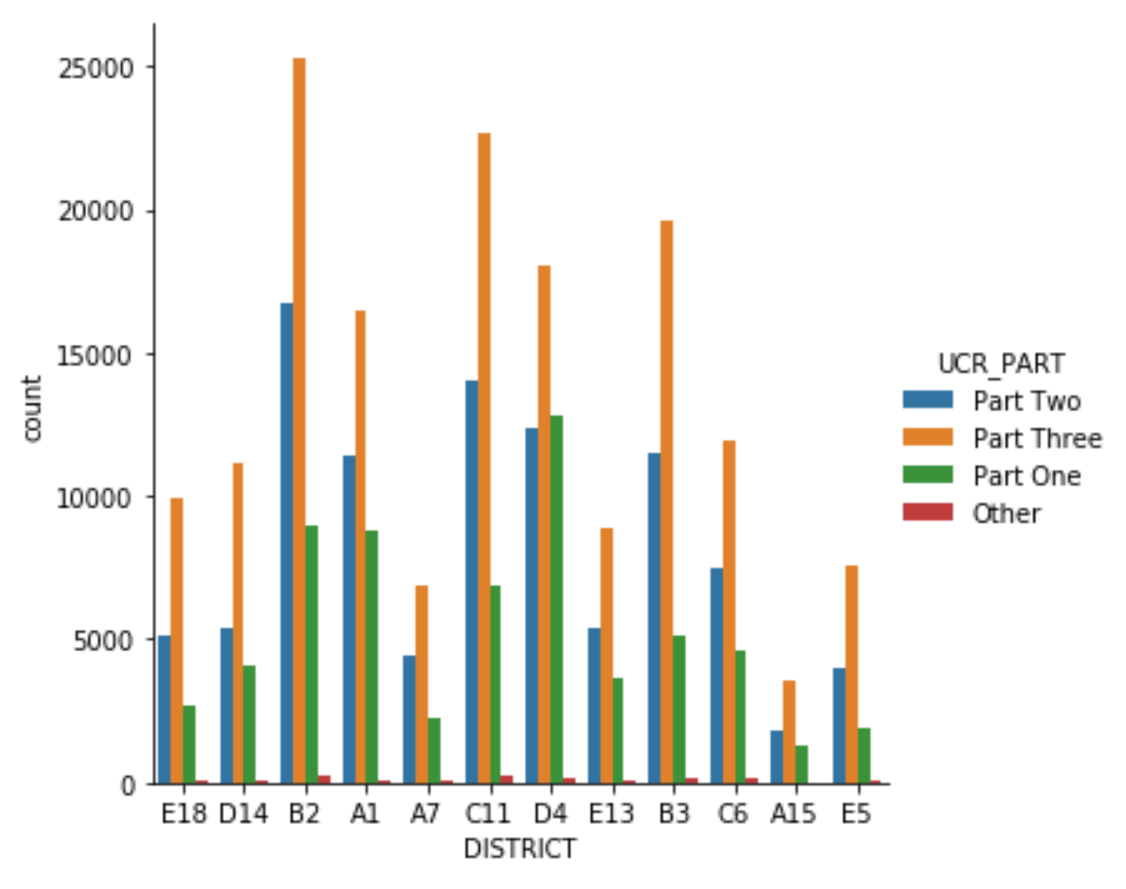
\includegraphics[scale = 2]{graph4paper1.png}

    A graph showing the police districts along with the amount of crime organized by UCR part number.
\end{center}
\section{Setup to our model}
\begin{itemize}
    \item Each location of city is organized by BPD districts
    \item 12 districts in total 
    \item Individual crimes are given an offense code number. These are then put into offense groups
    \item We predicted crimes based off of their offence group, not the individual offense code number
    \item 67 offense groups in total
    \item Combined the month and year columns to be one column
    \item One Hot encode all of our variables as they were categorical 
    \item Data was spilt into 80/20 training, testing datasets
\end{itemize}

%------------------------------------------------
\section{Decision Tree}
First we created a decision tree as a baseline for our data. To create this tree we used the DecisionTreeClassifier from sklearn. In order to get the maximum depth we ran the algorithm, testing depths from 1 to 119. A depth of 26 gave the highest accuracy. The accuracy for this model was low at only 0.18. This model misclassified a lot of the districts, for example it did not classify any of the A15 crimes correctly and classified a high amount of crimes as B2 when they should not have been.

\begin{center}
    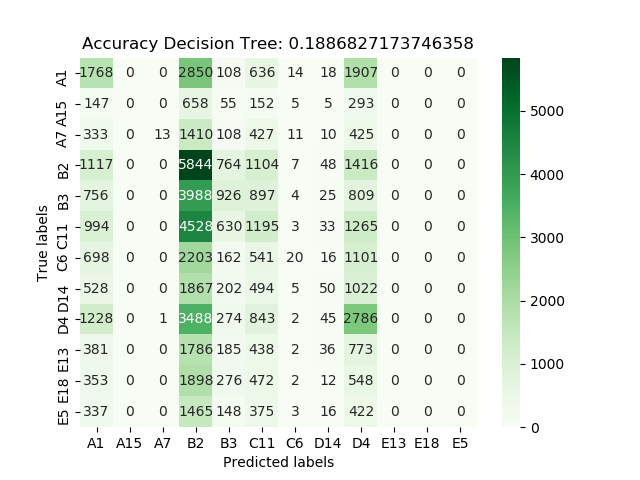
\includegraphics[scale = 2]{decision_tree_cm.png}
    
    A confusion matrix representing our decision tree model
\end{center}

\section{Multi-class logistic regression}
Next we created a multi-class logistic regression algorithm to try to compute where a crime was most likely to happen. To calculate the model, we used sklearn's built in LogisticRegression method.  This model had very low accuracy of about 20\% 
 \begin{center}
    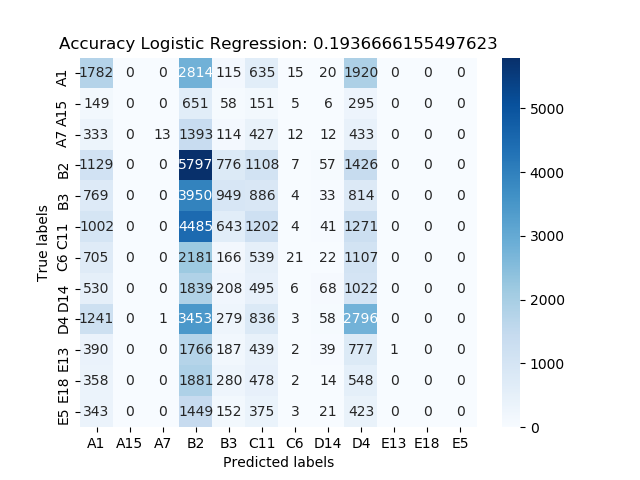
\includegraphics[scale = 2]{lr_cm.png}
  
       A Confusion Matrix representing our mutli-class logistic model
   \end{center}


  
%------------------------------------------------

\section{Visualizations}



\section{Future Work}
\begin{itemize}
    \item Increase prediction accuracy of our models
    \item Bring other data into consideration for classification such as time crime occurred
    \item Analyze other datasets for information on why certain districts have more crimes or are more likely to have specific crimes than other districts 
\end{itemize}
%%%%%%%%%%%%%%%%%%%%%%%%%%%%%%%%%%

\section*{Citations}

Jain, A. (2018, February). Crimes in Boston, Version 3. Retrieved November, 2019 from https://www.kaggle.com/ankkur13/boston-crime-data.\\
Boston Police. “The Boston Police Department's Virtual Community.” Bpdnews.com, 7 Dec. 2019, https://bpdnews.com/.




%\begin{theorem}[Baudoin, Gordina, M. 2018]
%If the operator $L$ satisfies 
%\[
%\Gamma_{2}^{L}(f)\geq\rho\Gamma^{L}(f),
%\]
%then the operator $\mathcal{L}$ satisfies the following generalized
%curvature-dimension inequality for any $f\in C^{\infty}\left(\mathbb{R}^{k}\times\mathbb{R}^{k}\right)$,
%\begin{align*}
%\Gamma_{2}(f) & \geq\left(\rho-\frac{C_{\sigma}}{2}\right)\Gamma(f)-\frac{C_{\sigma}}{2}\Gamma^{Z}(f),\\
%\Gamma_{2}^{Z}(f) & \geq0.
%\end{align*}
%
%\end{theorem}
%
%
%
%
%
%\begin{theorem}[Baudoin, Gordina, M. 2018]
%Let $P_{t}$ be the heat semigroup associated to $\mathcal{L}$. If
%$C_{\sigma}>2\rho$ and the operator $L$ satisfies 
%\[
%\Gamma_{2}^{L}(f)\geq\rho\Gamma^{L}(f),
%\]
%then for any $f\in C_{0}^{\infty}\left(\mathbb{R}^{k}\times\mathbb{R}^{k}\right)$,
%$t\geq0$ and $x\in\mathbb{R}^{k}\times\mathbb{R}^{k}$,
%\begin{align*}
% & \Gamma\left(P_{t}f\right)(x)+\frac{C_{\sigma}}{C_{\sigma}-2\rho}\Gamma^{Z}\left(P_{t}f\right)(x)\\
% & \leq e^{\left(C_{\sigma}-2\rho\right)t}\left(P_{t}\left(\Gamma(f)\right)+\frac{C_{\sigma}}{C_{\sigma}-2\rho}P_{t}\left(\Gamma^{Z}\left(f\right)\right)\right)(x).
%\end{align*}
%
%\end{theorem}
%
%
%
%We have the following Poincar\'e type inequality. 
%
%\begin{corollary}
%If $C_{\sigma}>2\rho$ then for any $f\in C_{0}^{\infty}\left(\mathbb{R}^{k}\times\mathbb{R}^{k}\right)$
%and $t\geq0$,
%\begin{align*}
% & P_{t}\left(f^{2}\right)-\left(P_{t}f\right)^{2}\\
% & \leq2\frac{e^{\left(C_{\sigma}-2\rho\right)t}-1}{C_{\sigma}-2\rho}\left(P_{t}\left(\Gamma(f)\right)+\frac{C_{\sigma}}{C_{\sigma}-2\rho}P_{t}\left(\Gamma^{Z}\left(f\right)\right)\right).
%\end{align*}
%\end{corollary}
%
%
%\item The results are more general, but constants aren't as sharp as the
%coupling technique.  
%\item The coupling technique yields a family of inequalities for $q\geq1$. 
%\end{itemize}












%%%%%%%%%%%%%%%%%%%%%%%%%%%%%%%%%%%%%%%%%%%%%%%%%%%%%%%%%%%%%%%%%






%\begin{thebibliography}{99}
%
%
%\bibitem{BGM2} Fabrice Baudoin, Maria Gordina, Phanuel Mariano, \emph{Gradient bounds for Kolmogorov type diffusions.} (2018), arXiv:1803.01436
%
%
%\end{thebibliography}




\end{multicols}
\vspace{1.5 in}


\end{document}
